\section{Results: predicting features}

\begin{frame}{7.1 - Results: feature}
	\begin{figure}[h]
	\centering
	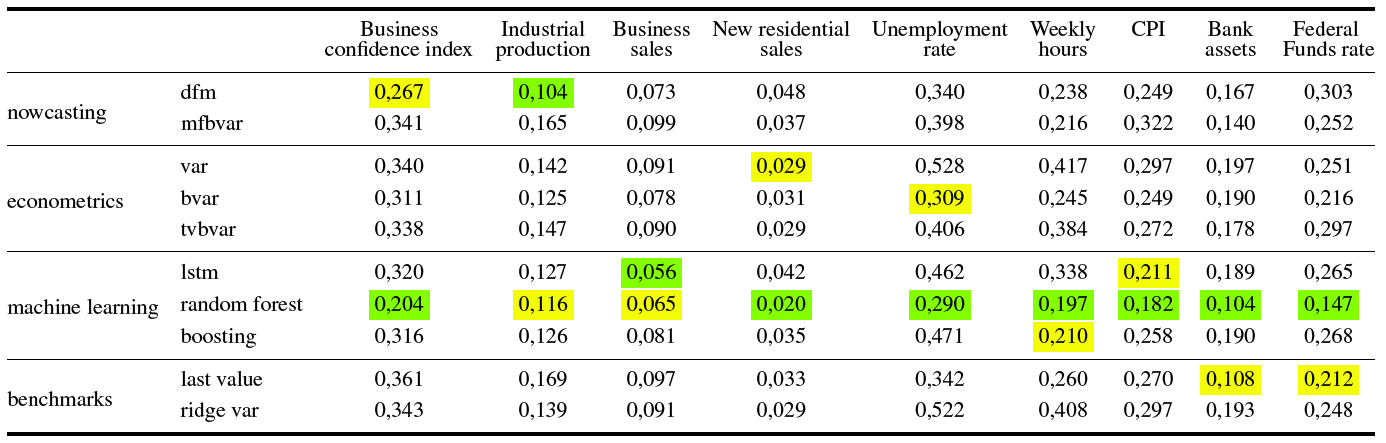
\includegraphics[width=1\linewidth]{im5}
	\caption{Feature nowcasts (1 quarter ahead)}
	\label{fig_71_1}
	\end{figure}
\end{frame}

\begin{frame}{7.1 - Results: feature}
\begin{figure}[h]
	\centering
	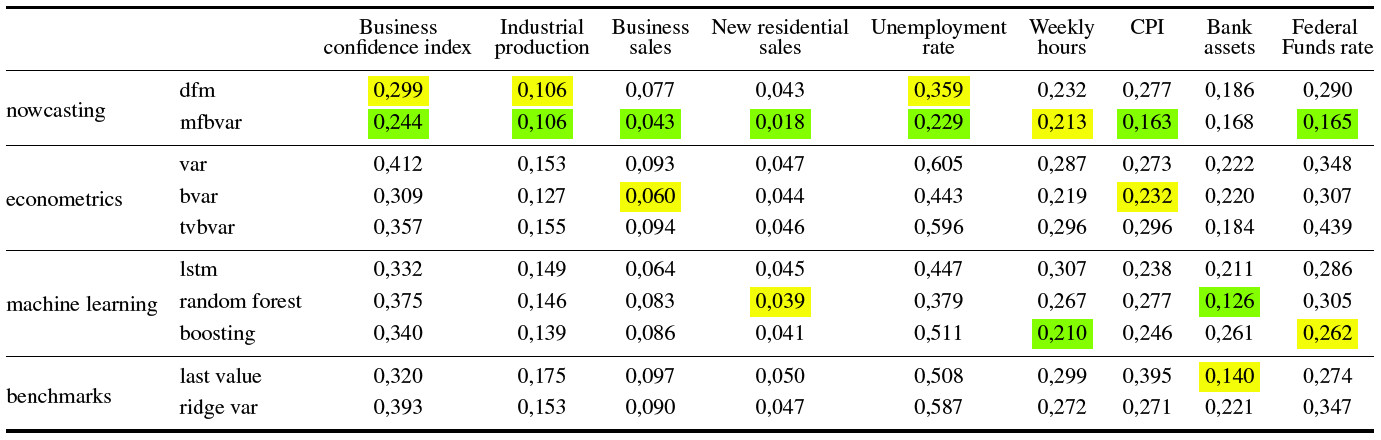
\includegraphics[width=1\linewidth]{im6}
	\caption{Feature forecasts (2 quarters ahead)}
	\label{fig_71_2}
\end{figure}
\end{frame}

\begin{frame}{7.1 - Results: feature}
\begin{figure}[h]
	\centering
	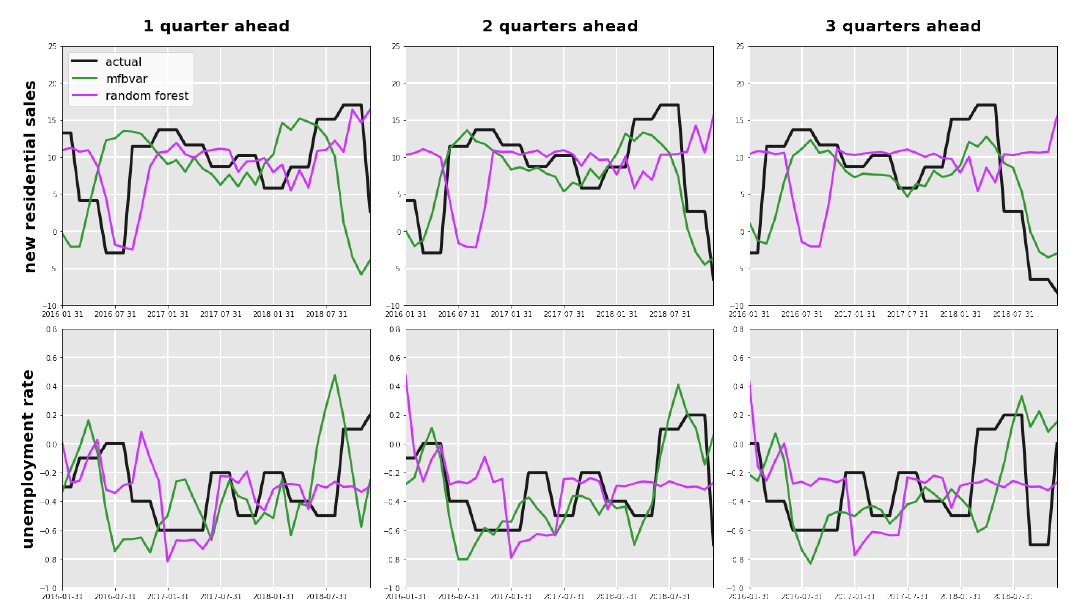
\includegraphics[width=1\linewidth]{im7}
	\caption{Feature forecasts (2 quarters ahead)}
	\label{fig_71_3}
\end{figure}
\end{frame}

\begin{frame}{7.2 - Conclusions: feature forecasts}
\begin{itemize}
	\item random forest is best for feature nowcasts
	\item MF-BVAR best at longer horizons
	\item for meaningful comparison: VAR on monthly sample, optimised dataset
	\item still difficult to understand why MF-BVAR anticipate dynamics
\end{itemize}	
\end{frame}

